\chapter{Simulating the Optimized Path}
\chaptermark{Simulation}

In this chapter paths the SITL simulater described in chapter \ref{ch:sim_env} will be used to fly an optimized path. Ideally the simulated model would be the Aerosonde UAV, as this is the model that has been used as the prediction model in the MPC. However, the ArduPilot SITL interface is only delivered with one default model to interface with JSBSim. This is a model of the Rascal110, and as there was no time to create a model of the Aerosonde the simulations will be performed with this model. Even though the results would have been more precise if the same model was used in both the optimization and the simulation, they will serve to show if the optimized path offer any improvements or not.

As mentioned in chapter \ref{ch:sim_env}, the guidance during simulations will be based on the LOS principle. By trial and failure the LOS distance was set to $150$m. The path flown by the UAV is shown together with the path that was tracked in Figure \ref{fig:sim_tracking}, and the results show that the tracking perfomance of the LOS guidance implemented in DUNE is satisfactory.

\begin{figure}
	\makebox[\textwidth][c]{
	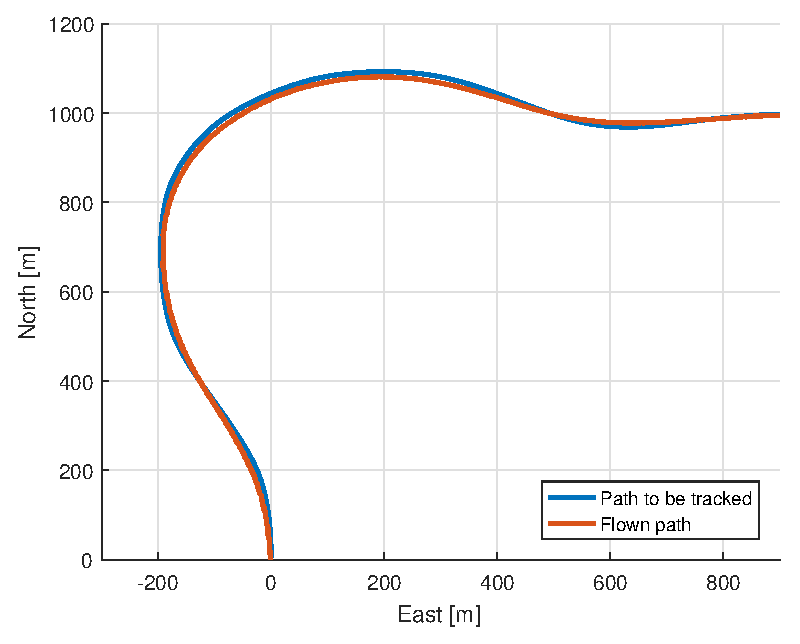
\includegraphics[width=0.8\textwidth, keepaspectratio=true]{../../results/sim/easy_path/fig_lin/tracking.eps}}
	\caption{Result when tracking the optimized path.}
	\label{fig:sim_tracking}
\end{figure}

\import{/}{gentle_path.tex}